% !TEX TS-program = pdflatex
% !TEX encoding = UTF-8 Unicode

% This is a simple template for a LaTeX document using the "article" class.
% See "book", "report", "letter" for other types of document.

\documentclass[12pt]{article} % use larger type; default would be 10pt

%\usepackage[utf8]{inputenc} % set input encoding (not needed with XeLaTeX)

%%% Examples of Article customizations
% These packages are optional, depending whether you want the features they provide.
% See the LaTeX Companion or other references for full information.

%%% PAGE DIMENSIONS

\usepackage{geometry} % to change the page dimensions
\geometry{a4paper} % or letterpaper (US) or a5paper or....
%\geometry{margins=2in} % for example, change the margins to 2 inches all round
% \geometry{landscape} % set up the page for landscape
%   read geometry.pdf for detailed page layout information
\usepackage{fullpage}
%\usepackage[top=tlength, bottom=blength, left=llength, right=rlength]{geometry}
%Edit individual page dimension variables described above, using the \addtolength and \setlength commands. For instance,
%\oddsidemargin=-1cm
%\setlength{\textwidth}{6.5in}
%\addtolength{\voffset}{-5pt}

\usepackage{graphicx} % support the \includegraphics command and options

% \usepackage[parfill]{parskip} % Activate to begin paragraphs with an empty line rather than an indent

%%% PACKAGES
\usepackage{booktabs} % for much better looking tables
\usepackage{array} % for better arrays (eg matrices) in maths
\usepackage{paralist} % very flexible & customisable lists (eg. enumerate/itemize, etc.)
\usepackage{verbatim} % adds environment for commenting out blocks of text & for better verbatim
%\usepackage{subfig} % make it possible to include more than one captioned figure/table in a single float

%\usepackage{caption}
\usepackage{subcaption}
\usepackage{cite}
\usepackage{graphicx}
\usepackage{hyperref,  mathrsfs, bm}

\usepackage{url}
%\renewcommand{\thesubfigure}{}
% justifying
\usepackage{ragged2e}
\usepackage{multirow}

\graphicspath{{./}{./../graphs/}{./graphs/}}


\usepackage{amssymb,amsmath,amsthm,amscd}

\usepackage[mathscr]{eucal}
%\usepackage[dvips]{graphicx}
%\usepackage{pstricks,pst-grad,pst-plot,pst-node}


%\usepackage{pgf}



%\newpsobject{showgrid}{psgrid}{subgriddiv=1,griddots=2,gridlabels=6pt}
\renewcommand{\raggedright}{\leftskip=0pt \rightskip=0pt plus 0cm}
% argmin
\DeclareMathOperator*{\argmin}{arg\,min}

\newcommand{\myred}{\color{red}}
\newcommand{\mygreen}{\color{green!50!black}}
\newcommand{\myblue}{\color{blue}}

\newcommand{\mcX}{\mathcal{X}}
\newcommand{\mcY}{\mathcal{Y}}
\newcommand{\mcG}{\mathcal{G}}
\newcommand{\mcF}{\mathcal{F}}


%\usepackage[tiling]{pst-fill}
\usepackage{epsfig}
\usepackage{graphicx}
\usepackage[usenames,dvipsnames]{color}

\usepackage{Sweave}
\usepackage{tikz}
\usepackage{pgf}

%%% HEADERS & FOOTERS
\usepackage{fancyhdr} % This should be set AFTER setting up the page geometry
\pagestyle{fancy} % options: empty , plain , fancy
\renewcommand{\headrulewidth}{0pt} % customise the layout...
\lhead{}\chead{}\rhead{}
\lfoot{}\cfoot{\thepage}\rfoot{}

%%% SECTION TITLE APPEARANCE
%\usepackage{sectsty}
%\allsectionsfont{\sffamily\mdseries\upshape} % (See the fntguide.pdf for font help)
% (This matches ConTeXt defaults)

%%% ToC (table of contents) APPEARANCE
\usepackage[nottoc,notlof,notlot]{tocbibind} % Put the bibliography in the ToC
\usepackage[titles,subfigure]{tocloft} % Alter the style of the Table of Contents
\renewcommand{\cftsecfont}{\rmfamily\mdseries\upshape}
\renewcommand{\cftsecpagefont}{\rmfamily\mdseries\upshape} % No bold!

\newtheorem{thm}{Theorem}
\newtheorem{cor}{Corollary}
\newtheorem{lem}{Lemma}
\newenvironment{remark}[1][Remark]{\begin{trivlist}
\item[\hskip \labelsep {\bfseries #1}]}{\end{trivlist}}




%%% END Article customizations

%%% The "real" document content comes below...

\title{ Fidelity-Commensurability Tradeoff in Joint Embedding of Disparate Dissimilarities}


%input affiliations


\author{Sancar Adali\thanks{Johns Hopkins University,
Department of Applied Mathematics and Statistics,
100 Whitehead Hall,
3400 North Charles Street,
Baltimore, MD 21218-2682} \and Carey E. Priebe\thanks{Johns Hopkins University,
Department of Applied Mathematics and Statistics,
100 Whitehead Hall,
3400 North Charles Street,
Baltimore, MD 21218-2682}
}
 

% \email{sadali1@jhu.edu}   %optional

% \email{cep@jhu.edu}   %optional


\begin{document}
\maketitle
\abstract{
}




\section{Introduction\label{sec:intro}}
% It is a challenge  to carry out inference on data from  disparate sources  (such as multiple sensors). The multitude  of sensors technology and large numbers of sensors  both  create difficulty and hold promise for efficient inference.
  We are interested in problems where the data sources are disparate and the inference task requires that the observations from  the different data sources  can be judged to be similar or dissimilar.
	
	Consider a collection of  English Wikipedia articles  and   French articles on the same topics. A pair of documents in different languages on the same topic are said to be ``matched". The ``matched'' wiki documents are  not necessarily direct translations of each other, so  we do not restrict ``matchedness'' to be a well-defined bijection between documents in different languages.
	%therefore the matchedness relation do not require  a bijection from the document space to another.
	However the matched ``documents''  provide examples of  ``similar"  observations coming from disparate sources, and we assume the training data consist of  a collection of ``matched'' documents.
	
  The inference task we consider is match detection, i.e. deciding whether a new English article and a new French article are on the same topic or not. While  a document in one language, say English, can be compared with other documents in English, a  French document  cannot be represented using the same features, therefore cannot be directly compared to English documents.  It is necessary   to derive a data representation  where the  documents from different languages can be compared (are commensurate).  %This data representation  should both preserve the high similarity of ``matched''  observations, the degree of  similarity of observations coming from the same source, and the dissimilarity of ``unmatched'' observations. 
	We will use a finite-dimensional Euclidean space for  this commensurate representation, where standard  statistical inference tools can be used.
  %It should also be parsimonius, so that it can be learned from data of limited  size.
	
     ``Disparate data''  means that  the observations are from  different ``conditions'', for example, the data might come from different type of sensors. Formally, the original data  reside in a heteregenous collection of  spaces.  In addition, the data might be structured and/or might reside in  infinite dimensional spaces. Therefore, it is possible that a feature representation of the data is not available or inference with such a representation is fraught with complications (e.g. feature selection, non-i.i.d. data, infinite-dimensional spaces). This motivates our  dissimilarity-centric approach. For an excellent resource on the usage of dissimilarities in pattern recognition, we refer the reader to the P\k{e}kalska and Duin book \cite{duin2005dissimilarity}.
		
		Since we proceed to inference starting from a dissimilarity representation of the data, our methodology may be applicable to any scenario in which multiple dissimilarity measures are available.  Some illustrative examples include:  pairs of images and their descriptive captions,  textual content  and  hyperlink graph
structure of  Wikipedia  articles, photographs taken under different illumination conditions. In each case, we have an intuitive notion of ``matchedness'': for photographs taken under different illumination conditions, ``matched'' means they are of the same person. For a collection of linked Wikipedia articles, the different conditions  are  the textual content and hyperlink graph structure, ``matched'' means a text document and  a vertex  in the graph corresponds to the same Wikipedia article. 

    To quantify how suitable the commensurate representation is for subsequent inference, two error criteria can be defined: \emph{fidelity}, which refers to how well the available dissimilarities in a condition are preserved and \emph{commensurability}, which refers to how well the dissimilarities between ``matched'' objects are preserved. These two concepts will be made concrete in a later section \ref{sec:FidComm}.

The major question  addressed in this paper is whether, in the tradeoff between fidelity and commensurability, there is a ``sweet spot'': increases in fidelity (or commensurability) do not result in superior performance for  the inference task, due to the resulting commensurability (or fidelity) loss. 
%The existence of such an extremum obviously depends on the inference task and the performance metric. Once  we define fidelity and commensurability errors, and the optimal tradeoff between the two,  interesting questions follow:  conditions for existence , conditions for uniqueness, the selection of an estimator for the extremum point.

    
 \begin{comment}
 The typical multiple sensor setting is visualized in  Figure ~\ref{fig:fig1}.
\begin{figure}
\centering
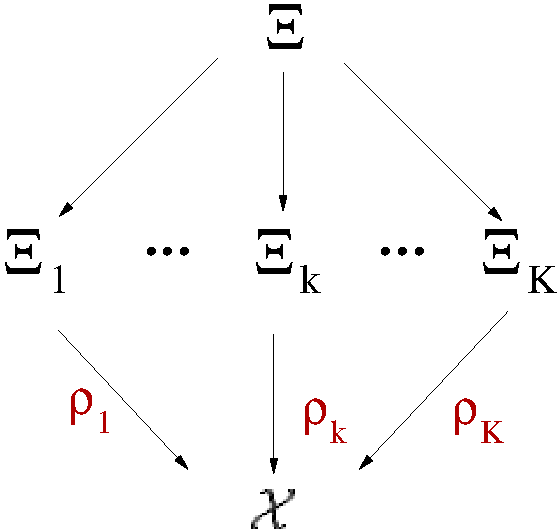
\includegraphics[scale=0.75]{gen-model-orig-proj.pdf}
\caption{Multiple Sensor setting}
\label{fig:fig1}
\end{figure}
\end{comment}


\section{Related Work \label{sec:RelatedWork}}
There have many efforts toward solving the related problem of ``manifold alignment". ``Manifold alignment" seeks to find correspondences between disparate datasets in different conditions (which are  sometimes referred as ``domains'') by aligning their underlying manifolds. The setting that is common in the literature  is the semi-supervised setting\cite{Ham2005a}, where  correspondences between two collections of points  are given and the task is to find correspondences between a new set of points in each condition. In contrast, the hypothesis testing task discussed in this paper is to determine whether any given pair of points is ``matched" or not. The proposed solutions\cite{Wang2008,Zhai2010,3wayNMDS}
 follow a common approach: they look for a common commensurate latent space such that the representations (either projections or embeddings) of the observations in this space match.

Wang and Mahedavan~\cite{Wang2008} suggest an  approach that uses embedding followed by Procrustes Analysis to find maps from the embedding spaces to a commensurate space. Given a paired set of points, Procrustes Analysis~\cite{Sibson}  finds a linear transformation from one set of points to the other that minimizes sum of squared distances between pairs. In the problem considered in \cite{Wang2008}, the paired set of points are low-dimensional embeddings of kernel matrices. For the embedding step, they chose to use Laplacian Eigenmaps, though their algorithm allows for any appropriate embedding method.

 Zhai et al.~\cite{Zhai2010}  solves an optimization problem  with respect to  two projection matrices for the observations in two domains.  The energy function that is optimized contains three terms: two \emph{manifold regularization terms} and one \emph{correspondence preserving term}. The  \emph{manifold regularization terms} ensure that the local neighborhood of points are preserved in the low-dimensional space, by making use of the reconstruction error for Locally Linear Embedding\cite{Roweis_LLE}.
The \emph{correspondence preserving term} ensures that ``matched'' points are mapped to proximate locations in the commensurate space.

Ham and Lee \cite{Ham2005a} solve the problem in the semi-supervised setting by a similar approach, by optimizing a energy function that has three terms that are analogous to the terms in ~\cite{Zhai2010}.
%to minimize three terms in an energy function %similar to the  JOFC approach (see Section \ref{sec:JOFC}). 
%One of the terms is the \emph{correspondence preserving term} which is the sum of the squared distances between corresponding points and is analogous to the commensurability error term in JOFC. The other two terms are \emph{manifold regularization terms} and consist of the reconstruction error for a Locally Linear Embedding of the projected points. These terms, analogous to fidelity, make sure the projections in the lower dimension retain the structure of the original points. For fidelity error terms in the JOFC setting, this is done by preserving dissimilarities. For manifold regularization terms, this is done by preserving the local neighborhood of points, such that close points are not mapped apart.
%Ham and Lee solve the problem in semi-supervised setting by a similar approach, by minimizing a cost function of three terms,






\begin{comment}
If the source of dissimilarities  are actually observations that are vectors in Euclidean space,  unless 
\begin{itemize}
\item the dissimilarity matrix is the Euclidean distance matrix of the original observations, and, 
\item the embedding dimension is greater or equal to the dimension of the original observations,
\end{itemize}
MDS with raw stress will not result in a perfect reconstruction  of the original observations. Note that the objective of the (joint) embedding is not \emph{perfect} reconstruction, but the best embedding for the exploitation task which is to test whether two sets of dissimilarities are ``matched". What is considered a ``good"'  representation will be dependent on how well the information in original dissimilarities that is relevant to the the match detection task is preserved. Fidelity and commensurability quantify this preservation of information.
\end{comment}


\section{Problem Description}
In the problem setting considered here,  $n$ different objects are measured under $K$ different conditions (corresponding  to, for example, $K$ different sensors). We assume we begin with dissimilarity measures. These will be represented in matrix form as $K$ $n \times n$ matrices $\{\Delta_k,k=1 ,\ldots,K\}$.  In addition, for each condition, dissimilarities between  a new object  and the previous 
$n$ objects $\{\mathcal{D}_k,k=1 ,\ldots,K\}$ are available. Under  the null hypothesis, these new dissimilarities represent a \emph{single} new object   measured under $K$ different conditions. Under the alternative hypothesis, the dissimilarities $\{\mathcal{D}_k\}$ represent \emph{separate} new objects   measured under $K$ different conditions~\cite{JOFC}. %The test dissimilarities are referred to as  out-of-sample (OOS) dissimilarities. 

For the English-French Wikipedia  article example in the introduction,  the dissimilarities between articles in the same language  ($\{\Delta_k\})$ are available. The dissimilarities between the new English article and the  other $n$ English articles $(\mathcal{D}_1)$ are also available, as well as the dissimilarities between the new French article  and the other $n$ French articles $(\mathcal{D}_2)$. The null hypothesis is that the new English and French articles are on the same topic, while the alternative hypothesis is that they are on different topics.

  In order to derive a data representation where dissimilarities from disparate sources ($\{\mathcal{D}_k\}$)  can be compared, the dissimilarities must be embedded in a commensurate metric space where the metric can be used to distinguish between matched and unmatched observations.


To embed multiple dissimilarities  $\{\Delta_k\}$  into a commensurate space, an omnibus dissimilarity matrix  $M \in \mathbb{R}^{nk \times nk}$  is constructed. Consider, for $K=2$,
 \begin{equation}
M=  \left[ \begin{array}{cc}
         \Delta_1 & L\\
        L^T  & \Delta_2 
     \end{array}  \right]     \label{omnibus} 
\end{equation} where $L$ is a matrix of imputed entries to be described later. 

\begin{remark}
For clarity of exposition,we will consider $K=2$; the generalization to $K>2$ is straightforward. 
\end{remark}

We define the commensurate space to be  $\mathbb{R}^d$, where the embedding dimension $d$ is pre-specified. The selection of $d$ -- model selection -- is  a task that requires much attention and is  beyond the scope of this article. Investigation of the effect of $d$ on testing performance will be pursued in a  subsequent paper.

 We use multidimensional scaling (MDS) \cite{borg+groenen:1997} to embed  the omnibus matrix in this  space, and obtain  a configuration of $2n$ embedded points $\{\hat{x}_{ik}; i=1,\ldots,n;k=1,2\}$ (which can be represented as $\hat{X}$, a $2n \times d$ matrix, where each row of the configuration matrix is the coordinate vector of an embedded point). The discrepancy between the interpoint distances of $\{\hat{x}_{ik}\}$ and the given dissimilarities in  $M$ is made as small  as possible, as measured by an objective function $\sigma(\widetilde{X};M)$ which will be described later. In matrix form, $$ \hat{X}=\arg \min_{\widetilde{X}} \sigma(\widetilde{X};M).$$ 
%This approach will be referred to as the Joint Optimization of Fidelity and Commensurability (JOFC) approach, for reasons that will be explained in \ref{sec:FidComm}. 

\begin{remark} 
We will use $x_{ik}$ to denote the (possibly notional)  observation  for the $i^{th}$ object in the $k^{th}$ condition, $\tilde{x}_{ik}$ to denote an argument of the objective function  and  $\hat{x}_{ik}$  to denote the $\arg\min$  of the objective function. The notation for matrices ($X,\widetilde{X},\hat{X}$) follows the  same convention.
\end{remark}

  Given the omnibus matrix $M$ and the $2n \times d$ embedding configuration matrix $\hat{X}$ in the commensurate space, the out-of-sample extension~\cite{TrossetOOS} for MDS will be used to embed the test dissimilarities $\mathcal{D}_1$ and $\mathcal{D}_2$.  Once the test similarities are embedded as two points ($\hat{y}_{1},\hat{y}_{2}$) in  the commensurate space, it is possible to  compute the test statistic \[
\tau=d\left(\hat{y}_{1},\hat{y}_{2}\right)\label{teststat}
\] for the two ``objects'' represented by  $\mathcal{D}_1$ and $\mathcal{D}_2$.  For large values of $\tau$, the null hypothesis will be rejected. 
   If  dissimilarities between matched objects are smaller than dissimilarities between unmatched objects with large probability, and the embeddings preserve this stochastic ordering,  we could reasonably expect the test statistic to yield large  power. 
\section{Fidelity and Commensurability\label{sec:FidComm}}



Regardless of the inference task,  to expect reasonable performance from the embedded data in the commensurate space, 
%we have to use both the original dissimilarity information in each separate condition \emph{and}  the matchedness of dissimilarities. 
it is necessary to pay heed to these two error criteria: %adhered to:

\begin{itemize}
\item Fidelity describes how well the mapping to commensurate space preserves the original dissimilarities. The \emph{loss of fidelity} can be measured with the  within-condition \emph{ fidelity error}, given by
    \[
\epsilon_{f_{(k)}} = \frac{1}{{{n}\choose{2}}} \sum_{1 \leq i < j \leq n} (d(\widetilde{\bm{x}}_{ik},\widetilde{\bm{x}}_{jk})-\delta_{ijkk})^2
.\] 
Here $\delta_{ijkk}$ is the dissimilarity between the $i^{th}$ object and the $j^{th}$ object where both objects are in the $k^{th}$  condition, and $\widetilde{\bm{x}}_{ik}$ is the embedded representation of the $i^{th}$ object  for the $k^{th}$ condition;  $d(\cdot,\cdot)$ is the Euclidean distance function.

\item Commensurability describes how well the mapping to commensurate space preserves matchedness of matched observations. The \emph{loss of commensurability} can be measured by the between-condition {\em commensurability error} which is given by
    \[
\epsilon_{c_{(k_1,k_2)}} = \frac{1}{n} \sum_{1 \leq i \leq n;k_1 <k_2} (d(\widetilde{\bm{x}}_{ik_1},\widetilde{\bm{x}}_{ik_2})- { \delta_{iik_1k_2}})^2
\label{comm-error}
\]
 for conditions $k_1$ and $k_2$; $\delta_{iik_1k_2}$  is the dissimilarity between the $i^{th}$ object under  conditions   $k_1$ and  $k_2$. 
Although  the between-condition dissimilarities of the same object, ${ \delta_{iik_1k_2}}$, are not available,  it is reasonable to set these dissimilarities to $0$ for all $i,k_1,k_2$. These dissimilarities correspond to  diagonal  entries of the  submatrix $L$ in  the omnibus matrix  M in equation \eqref{omnibus}. Setting these diagonal entries to $0$ forces matched observations to be embedded close to each other. \label{commens}  
\end{itemize}

While  the above expressions for  \emph{fidelity} and  \emph{commensurability} errors  are specific to the joint embedding of disparate dissimilarities, the concepts of fidelity and commensurability are  general enough to be applicable to other dimensionality reduction methods for data from disparate sources. 

 In addition to fidelity and commensurability, there is the \emph{separability} criteria:  dissimilarities between unmatched  observations in different conditions  should be preserved (so that unmatched pairs are not embedded close together).  The error for this criteria can be measured by  $\epsilon_{s_{k_1k_2}} = \frac{1}{{{n}\choose{2}}} \sum_{1 \leq i < j \leq n;k_1 <k_2} (d(\widetilde{\bm{x}}_{ik_1},\widetilde{\bm{x}}_{jk_2})-{ \delta_{ijk_1k_2}})^2$ for  conditions   $k_1$ and  $k_2$.

Let us now show how fidelity and commensurability errors  can be made explicit in the objective function. Consider the weighted raw stress criterion ($\sigma_{W}(\cdot)$) which we choose as the objective function for the embedding  of  $M$. The entries of $M$ are $\delta_{ijk_1k_2}$ for the available dissimilarities. As the between-condition dissimilarities, 
$\delta_{ijk_1k_2}$ for $i\neq j$, are  not available in general, the entries corresponding to the unavailable dissimilarities can be imputed as $\delta_{ijk_1k_2}=\frac{\delta_{ijk_1k_1}+\delta_{ijk_2k_2}}{2}$.
\begin{equation}
\sigma_{W}(\widetilde{X};M)=\sum_{i\leq j,k_1\leq k_2} {w_{ijk_1k_2}(D_{ijk_1k_2}(\widetilde{X})-\delta_{ijk_1k_2})^2  }\label{raw-stress}.
\end{equation}
 Here, $ijk_1k_2$ subscript of a partitioned matrix refers to the entry in the $i^{th}$ row and $j^{th}$ column of the sub-matrix in $k_1^{th}$ row partition and $k_2^{th}$ column partition, $W$ is the weight matrix, $\widetilde{X}$ is the configuration matrix that is the argument of the stress function, $D$ is the Euclidean distance function of the rows of its matrix argument.   \emph{Each of the individual terms in the sum \textrm{(\ref{raw-stress})} can be ascribed to fidelity, commensurability or separability}. %\footnote{\delta_{ijk_1k_2} is just a reindexing of M_{st}, k_1,k_2 are row/column indices of the block matrix (i,j)  are  row/column indices of the matrix entry, },

\begin{comment}
\begin{align}
\sigma_W(\cdot;M)  &= & &\sum_{i\leq j,k_1\leq k_2} {w_{ij{k_1}{k_2}}(d_{ij{k_1}{k_2}}(\cdot)-\delta_{ijk_1k_2})^2 }_{term with indices {i,j,k_1,k_2}} \notag\\
\hspace{3pt} &=& &\underbrace{\sum_{i=j,k_1<k_2}  {w_{ij{k_1}{k_2}}(d_{ij{k_1}{k_2}}(\cdot)-\delta_{ijk_1k_2})^2}}_{Commensurability}  \hspace{10pt}  &  + &\hspace{2.5em} \underbrace{\sum_{i<j,k_1=k_2}  {w_{ij{k_1}{k_2}}(d_{ij{k_1}{k_2}}(\cdot)-\delta_{ijk_1k_2})^2  }  } _{Fidelity}\notag\\
\hspace{3pt}&+&  &\underbrace{\sum_{i< j,k_1<k_2}  {w_{ij{k_1}{k_2}}(d_{ij{k_1}{k_2}}(\cdot)-\delta_{ijk_1k_2})^2  }  } _{Separability}\label{eq:FidCommSep}\hspace{10pt} .
\end{align}

\end{comment}

\begin{align}
\sigma_W(\cdot;M)  &=  \sum_{i,j,k_1,k_2} \underbrace{{w_{ij{k_1}{k_2}}(D_{ij{k_1}{k_2}}(\cdot)-M_{ijk_1k_2})^2 }}_{term_{i,j,k_1,k_2}}  & \notag\\
\hspace{3pt} &=  \underbrace{\sum_{i=j,k_1<k_2}  term_{i,j,k_1,k_2}}_{Commensurability}  \hspace{10pt}    +  \underbrace{\sum_{i<j,k_1=k_2}   term_{i,j,k_1,k_2}  } _{Fidelity}
\hspace{3pt}+  \underbrace{\sum_{i< j,k_1<k_2}  term_{i,j,k_1,k_2}  } _{Separability}\label{eq:FidCommSep}\hspace{10pt} &.
\end{align}

   Due to the fact that data sources are ``disparate", it is not obvious how  a dissimilarity between an object in one condition and another object in another condition  can be computed or  defined in a sensible way. Although these unavailable dissimilarities can be imputed as mentioned,  they can  also be set to any finite number and ignored in the embedding by setting the associated weights in the raw stress function to be 0 for the weighted raw stress criterion. We choose to do the latter to  restrict our attention to  the fidelity-commensurability tradeoff. 
 %

 As mentioned in description of commensurability, we set the between-condition dissimilarities of the same object ($\{M_{iik_1k_2}\}$) to $0$. Then the raw stress function can be written as
\begin{align}
\sigma_W(\widetilde{X};M)\hspace{3pt}   
\hspace{3pt}&=&\underbrace{\sum_{i=j,k_1< k_2}  {w_{ij{k_1}{k_2}}(D_{ij{k_1}{k_2}}(\widetilde{X}))^2}}_{Commensurability}  \hspace{10pt}  &  +&\underbrace{\sum_{i< j,k_1=k_2}  {w_{ij{k_1}{k_2}}(D_{ij{k_1}{k_2}}(\widetilde{X})-M_{ijk_1k_2})^2  }  } _{Fidelity}\notag\label{eq:FidCommSep}\hspace{10pt} .
\end{align}
This motivates  the naming of the   omnibus embedding approach as Joint Optimization of Fidelity and Commensurability (JOFC).



 The weights in the raw stress function allow us to address the question of the ``sweet spot'' in Fidelity-Commensurability tradeoff. Let $w \in (0,1)$. Setting the weights ($w_{ijk_1k_2}$)  for the commensurability  and fidelity  terms    to $w$ and $1-w$, respectively,  will allow us to control the relative importance of fidelity and commensurability terms in the objective function.

 Let us denote the raw stress function with these simple weights by $\sigma_w(\widetilde{X};M)$. With simple weighting, when $w=0.5$, all terms in the objective function have the same weights. We will refer to this weighting scheme as \emph{uniform weighting}. Uniform weighting does not necessarily yield the best fidelity-commensurability tradeoff in terms of subsequent inference. 

 Previous investigations of the JOFC approach \cite{JOFC} did not consider the effect of non-uniform weighting.
Our thesis is that using non-uniform weighting  in the objective function will allow for superior performance.
That is, for a given exploitation task there is an optimal $w$, denoted $w^*$, and in general $w^* \neq 0.5$.
In particular, we consider hypothesis testing, as in \cite{JOFC},
and we let the area under the ROC curve, $AUC(w)$, be our measure of performance for any $w \in [0,1]$.
In this case, we show that $AUC(w)$ is continuous, and hence $w^* = \arg\max_{w \in [0,1]} AUC(w)$ exists.
We demonstrate the potential practical advantage of our weighted generalization of JOFC via simulations.

 
\begin{comment}
 ``Conditions" and ``matched" refer to concepts dependent on the context of the  problem. Conditions could be different modalities of data, e.g., one condition could be  an image of an object, while the other condition could be a text description of the object. ``Matched", in general, means observations of the same object, or realizations of a common concept. 
 \end{comment}




\section{Definition of  $w^{*}$}
\begin{comment}
Suppose the dissimilarities we are given are distances for $n$ pairs of matched observations in $\mathbb{R}^p$.  Additionally, two pairs of dissimilarities, one for a matched pair, $\{y_{1}^{(m)} ,y_{2}^{(m)}\}$
 and another for an unmatched pair $\{y_{1}^{(u)} ,y_{2}^{(u)}\}$~\footnote{\! $^{(m)}$ is shorthand for ``matched'', $^{(u)}$ is shorthand for ``unmatched''} are available.
We embed two dissimilarity matrices, \[
 \Delta^{(m)} =D \left(\left[
\begin{array}{c}
\mathcal{T} \\
y_{1}^{(m)} \\
y_{2}^{(m)} 
\end {array}
\right]
\right)
 \hspace{1em} \textrm { and } \hspace{1em}
\Delta^{(u)} =D \left(\left[
\begin{array}{c}
\mathcal{T}\\
y_{1}^{(u)} \\
y_{2}^{(u)}
\end {array}
\right]\right) 
\]
which are two matrix-valued random variables : $\Delta^{(m)}:\Omega \rightarrow \mathbf{M}_{(2n+2)\times (2n+2)} $, $\Delta^{(u)}:\Omega \rightarrow \mathbf{M}_{(2n+2)\times (2n+2)} $  for the appropriate sample  space $(\Omega)$. $\mathcal{T}$ is a random ($2n \times p$) matrix containing a sample of  $n$ i.i.d.  pairs of  matched observations in $\mathbb{R}^p$.
\end{comment}
Let us denote the test dissimilarities ($\mathcal{D}_1$,$\mathcal{D}_2$)  by  ($\mathcal{D}_1^{(m)}$,$\mathcal{D}_2^{(m)}$)  under ``matchedness'' hypothesis, and  by ($\mathcal{D}_1^{(u)}$,$\mathcal{D}_2^{(u)}$)  under the alternative. The out-of-sample embedding of ($\mathcal{D}_1^{(m)}$,$\mathcal{D}_2^{(m)}$) involves the  augmentation of  the omnibus matrix $M$, which consists of $n$ ``matched''  pairs of dissimilarities,  with ($\mathcal{D}_1^{(m)}$,$\mathcal{D}_2^{(m)}$). The resulting augmented  $(2n+2)\times (2n+2)$ matrix  has the form:

 \begin{equation}
\Delta^{(m)}=  \left[ \begin{array}{cccc}
          \multicolumn{2}{c}{\multirow{2}{*}{\Huge{$M$}}} &  \mathcal{D}_1^{(m)} &\vec{\mathcal{D}}_{NA}\\
        & &  \vec{\mathcal{D}}_{NA}   & \mathcal{D}_2^{(m)} \\
				\mathcal{D}_1^{(m)T} & \vec{\mathcal{D}}_{NA}^T  &  0 & \mathcal{D}_{NA} \\
         \vec{\mathcal{D}}_{NA}^T & \mathcal{D}_2^{(m)T} & \mathcal{D}_{NA} &0\\
     \end{array}  \right].     \label{aug_omnibus} 
\end{equation}  where
the scalar $\mathcal{D}_{NA}$ and   the  vector of length $n$ $\vec{\mathcal{D}}_{NA}$   represent dissimilarities that are not available. 
In our JOFC procedure, these unavailable entries in $\Delta^{(m)}$ are either  ignored in the embedding optimization or imputed using other dissimilarities that are available. For a simpler  notation, let us assume it is the latter case. Also note that $\Delta^{(u)}$  has the same form as $\Delta^{(m)}$ where $\mathcal{D}_k^{(m)}$ is replaced by $\mathcal{D}_k^{(u)}$.

We define the dissimilarity matrices \{$\Delta^{(m)}$,$\Delta^{(u)}$\} to be  two matrix-valued random variables~: $\Delta^{(m)}:\Omega \rightarrow \mathbf{M}_{(2n+2)\times (2n+2)} $ and  $\Delta^{(u)}:\Omega \rightarrow \mathbf{M}_{(2n+2)\times (2n+2)} $) for the appropriate sample  space $(\Omega)$.
\begin{remark}
Suppose the objects in $k^{th}$  condition  can be represented as points in a measurable space $\Xi_k$, and the dissimilarities in $k^{th}$ condition are given by  a dissimilarity measure $\delta_k$ acting on pairs of points in $\Xi_k$. Assume $\mathcal{P}_{(m)}$ is the joint probability distribution over ``matched'' objects, while the joint distribution of ``unmatched'' objects \{$k=1,\ldots,K$\}  is $\mathcal{P}_{(u)}$. Assuming the data are i.i.d., under the two hypotheses (``matchedness'' and ``unmatchedness'', respectively), the $n+1$ pairs of objects are governed  by the product distributions $\{\mathcal{P}_{(m)}\}^n \times \mathcal{P}_{(m)} $ and $\{\mathcal{P}_{(m)}\}^n \times \mathcal{P}_{(u)} $.  The distributions of $\Delta^{(m)}$ and $\Delta^{(u)}$ are the induced probability distributions of  these product distributions (induced by the  dissimilarity measure $\delta_k$ applied to  objects in $k^{th}$ condition \{$k=1,\ldots,K$\})  .
\end{remark}


%is embedded in $d$-dimensional space with the constraint that the embedding of the first $2n$ points is the same as the embedding of $M$:


 The criterion function for the embedding is $\sigma_W(\widetilde{X};M)$ which can be written as $f_w(\widetilde{X},\Delta)$ for the simple weighting scheme with $w$, and an omnibus dissimilarity matrix $\Delta$. The embedding coordinates for the unmatched pair are  ${\hat{y}_{1}^{(u)},\hat{y}_{2}^{(u)}}$ where
 \[
{\hat{y}_{1}^{(u)},\hat{y}_{2}^{(u)}}
=\argmin_{\widetilde{y}_{1}^{(u)}, \widetilde{y}_{2}^{(u)}}\left[\min_{\widetilde{\mathcal{T}}}
{f_w\left(
\left[
\begin{array}{c}
{\widetilde{\mathcal{T}}} \\
\widetilde{y}_{1}^{(u)} \\
\widetilde{y}_{2}^{(u)}
\end {array}
\right]
,
\Delta^{(u)}
\right)
}
\right].
\]
A similar expression gives the embedding for the matched pair.
\begin{remark}
 Note that the in-sample embedding of $\widetilde{\mathcal{T}}$ is necessary but irrelevant for the inference task, hence the minimization with respect to $\widetilde{\mathcal{T}}$ is denoted by  $\min$ instead $\argmin$.
\end{remark}
\begin{remark}
 Note also that  all of the random variables following the embedding, such as $\hat{y}_{1}^{(u)}\!$,  are dependent on $w$; for the sake of simplicity, this will not be shown in the notation. 
\end{remark}

 Assuming $\Delta^{(m)} \rightarrow  \{\hat{y}_{1}^{(m)},\hat{y}_{2}^{(m)}\!\}$  and $\Delta^{(u)}\rightarrow \{\hat{y}_{1}^{(u)} , \hat{y}_{2}^{(u)}\}$ are measurable maps, consider the test statistic $\tau$ which equals $d(\hat{y}_{1}^{(m)},\hat{y}_{2}^{(m)})$ under null hypothesis of matchedness and $d(\hat{y}_{1}^{(u)},\hat{y}_{2}^{(u)})$ under alternative. Under the null hypothesis, the distribution of the statistic is governed by the distribution of $\hat{y}_{1}^{(m)}$ and $\hat{y}_{2}^{(m)}$, under the alternative it is governed by  the distribution of $\hat{y}_{1}^{(u)}$ and $\hat{y}_{2}^{(u)}$.

 Then, $\beta\left( w,\alpha\right)=1-F_{d \left(\hat{y}_{1}^{(u)},\hat{y}_{2}^{(u)}\right)}(F_{d\left(\hat{y}_{1}^{(m)},\hat{y}_{2}^{(m)}\right)}^{-1}(1-\alpha))$ where $F_Y$ denotes  the   cumulative distribution function of  $Y$.
The AUC function is defined as:  $$AUC(w)=\int_{0}^{1}\! \beta\left( w,\alpha\right)\,\mathrm{d}\alpha \; .$$
%\footnote{
Although we might care about optimal $w$ with respect to  $\beta\left( w,\alpha\right)$ (with a fixed type I error rate $\alpha$),  it will be more convenient to define $w^*$ in terms of the AUC function.
%}

 Finally, define $$w^{*}=\arg\max_w{AUC\left( w\right)}. $$

\begin{comment}
Given  specific distributions $\mathbf{F}_{ \hat{y}_{k}^{(m)}}$,$\mathbf{F}_{ \hat{y}_{k}^{(u)}}$,   $w^*$ must be defined with respect to the value of allowable type I error rate $\alpha$.  For two different $\alpha$ values, it is quite possible that $\beta_{\alpha_1}(w_1)>\beta_{\alpha_1}(w_2)$  and $\beta_{\alpha_2}(w_1)<\beta_{\alpha_2}(w_2)$. This can be observed in results in Section \ref{sec:Simulation Results}.  
\end{comment}
 Some important questions about $w^*$ are  related to the nature of the AUC function.
While finding an analytical expression for the value of $w^*$ is intractable, an estimate $\hat{w}^*$  based on  estimates of $AUC(w)$ %$\beta_{\alpha}(w^*)$
 can be computed.  For the Gaussian setting described in \ref{subsec:GaussianSet} , a Monte Carlo simulation is run in  Section  \ref{sec:Simulation Results} to find the estimate of $AUC(w)$ for different $w$ values.
% $\beta_{\alpha}\left( w\right)$  at various values of $\alpha$ , 
%which can be used to compute  values .

\begin{comment}
A closed-form expression for this function will be hard to find  even in the most simple of cases. So consider the estimate from the Monte Carlo simulation $\beta^{(m)}_{\alpha}(w)$ for the estimate computed from $2m$ testing pairs, m matched pairs and m unmatched pairs. In addition, consider an arbitrary element $\omega$ of sample space $\Omega$. By law of large numbers, $\beta^{(m)}_{\alpha}\rightarrow\beta_{\alpha}(w)$ pointwise.  We will omit $w$ from the expressions of the functions. Suppose the test statistic values  are $T_0^{i}$, $T_A^{i}$ $i=1,\ldots,m$  respectively for matched and unmatched test pairs. Note that $\beta^{(m)}_{\alpha}$ can be written as $\sum_{j=1}^m I(T_A^{j}>T_0^{(i)})$ where $T_0^{(i)}$ is the $i=\lceil {m*(1-\alpha)} \rceil^{th}$ order statistic of $T_0^{i},i=1,\ldots,m$. Replacing the indicator function with the unit step function
\[
\beta^{(m)}_{\alpha}=\sum_{j=1}^m u(T_A^{j}-T_0^{(i)})
\]

Instead of this function which is not differentiable with respect to  $T_0^{i}$ and  $T_A^{i}$, consider the ``soft" approximation of this function with the sigmoid function
\[
\mathcal{B}_{alpha}^{(m)}=\sum_{j=1}^m \sigma(T_A^{j}-T_0^{(i)})
\]

Now we can consider the derivative  $\frac{d\mathcal{B}_{\alpha}^{(m)}}{dw}$, which is equal to 
\[
\frac{d\mathcal{B}_{\alpha}^{(m)}}{dw}=\sum_{j=1}^m \frac{\partial \sigma(T_A^{j}-T_0^{(i)})}{\partial T_A^{j}} \frac{\partial T_A^{j}}{w}+ \sum_{j=1}^m \frac{\partial \sigma(T_A^{j}-T_0^{(i)})}{\partial T_0^{j}} \frac{\partial T_0^{j}}{\partial w}
\] if the partial derivatives exist.
To prove differentiability of $\beta_{\alpha}\left( w\right)$ , we refer to Theorem 5.3.3 in \cite{ElClassAnalysis-5-3-3}, which requires the pointwise convergence of   $\mathcal{B}_{alpha}^{(m)}$   to  $\beta_{\alpha}\left( w\right)$ , that $\frac{d\mathcal{B}_{alpha}^{(m)}}{dw}$ are continuous and that they  converge \emph{uniformly} to a function $g$. Since the sigmoid function $\sigma(\cdot)$ is continously differentiable, we can focus on our attention  on $ \frac{\partial{T_0^{j}}}{\partial{w}}$ and $ \frac{\partial{T_0^{j}}}{\partial{w}}$. We show  that while the embedded configurations of points might not be  continuous everywhere (we present a particular example in \ref{subsubsec:Discontinuity}) $T_0^{j}$ and $T_A^{i}$ is nevertheless continuous with respect to $w$. 
\end{comment}


 
\subsection{Continuity of $AUC(\cdot)$} 
 Let $T_0(w)=d(\hat{y}_{1}^{{(m)}},\hat{y}_{2}^{{(m)}})$ and $T_a(w)=d(\hat{y}_{1}^{(u)},\hat{y}_{2}^{(u)})$ denote the value of the test statistic under null and alternative distributions  for the embedding with the simple weighting $w$.  %stochastic process whose sample path is  a function of $w$ where the randomness comes from $\Delta^{(m)}$, $\Delta^{(u)}$ and %$\mathcal{T}$ . 
%Consider $\beta_{\alpha}(\cdot)$ as a function of $w$, which can be written as $P\left[T_a(\cdot)>c_{\alpha}(\cdot)\right]$ where $c_{\alpha}(\cdot)$ is the critical value for level $\alpha$. Instead of  $\beta_{\alpha}(\cdot)$  
The area under the curve measure can be written as: $$AUC(w)=P\left[T_a(w)>T_0(w)\right]$$ where $T_a(\cdot)$ and $T_0(\cdot)$  can be regarded as  stochastic processes whose sample paths are functions  of $w$. We prove $AUC(w)$ is continous with respect to $w$.
% except at a finite number of points in $(0,1)$.
We start with this lemma from \cite{Raik1972}.

\begin{lem}
Let $z$ be a random variable. The functional $g(z;\gamma) = P\left[z \geq \gamma \right]$ is upper semi-continuous in probability with respect to $z$ . Furthermore, if $P\left[z = \gamma \right]=0$, $g(z;\gamma)$ is continuous in probability with respect to $z$. \label{lemma_1}
\end{lem}

\begin{proof}
Suppose $z_n$ converges to $z$ in probability. Then by definition, for any  $\delta>0$ and  $\epsilon>0$, $\exists	N$ such that for all   $n>N$ 
$$ Pr\left[\left|z_n-z\right| \geq \delta \right] \leq \epsilon.$$

 The functional  $g(z;\gamma)$ is  non-increasing and left continuous with respect to $\gamma$. Therefore, for $\delta>0$, 
$g(z_n;\gamma) -g(z;\gamma) \geq g(z_n;\gamma) -g(z;\gamma-\delta) $ and due to the left-continuity, the difference between the two sides of the inequality can be made as small as desired.

\begin{eqnarray}
g(z_n;\gamma) - g(z;\gamma-\delta) & = &Pr\left[z_n\geq \gamma \right] -Pr\left[z \geq  \gamma - \delta \right] \label{prob_defn}\\
& \leq &  Pr\left[\{z_n \geq \gamma \} \backslash \{z \geq \gamma - \delta \} \right] \label{set_diff}\\
& \leq & Pr\left[\{\{z_n \geq \gamma \} \backslash \{z \geq \gamma - \delta \} \} \cap \{z_n \geq  z\} \right] \label{conjunct_with_set} \\
& =  & Pr\left[\{z_n - z \geq \delta \} \right] \leq \epsilon \label{upper_semicont}
\end{eqnarray}
 
Since $\epsilon$ and $\delta$ are arbitrary,
 $ \limsup_{n \rightarrow \infty} ( {g(z_n;\gamma)}- g(z;\gamma) ) =  0$ for any $\delta>0, $ i.e. $g(z;\gamma)$ is upper semi-continuous .

By arguments  symmetric to  \eqref{prob_defn}-\eqref{upper_semicont} , we can show that

\begin{equation}
g_(z;\gamma+\delta) - g(z_n;\gamma) \leq \epsilon \label{lower_semicont}
\end{equation}


In addition , assume that  $P\left[z = \gamma \right]=0$, then $g(z;\gamma)$ is also right-continuous with respect to $\gamma$. Therefore, 
$g(z_n;\gamma) -g(z;\gamma) \leq g(z_n;\gamma) -g(z;\gamma+\delta)$ and the difference can be made as small as possible. Along with \ref{lower_semicont}, this means that

 \[ 
\liminf_{n \rightarrow \infty} ( {g(z_n;\gamma)}- g(z;\gamma) ) = 0. 
\] Therefore , $\lim_{n\rightarrow \infty}g(z_n;\gamma) = g(z;\gamma)$ ,i.e. $g(z;\gamma)$ is continuous in probability with respect to $z$.
\end{proof}

\begin{thm}
Let $T(w,\omega)$ be continuous with respect to $w$ at $w_0$  for almost all $\omega$ and let $T(w_0,\omega)$ be measurable map $\Omega \rightarrow \mathbb{R}$, then $F_{\gamma}(w)=Pr\left[T(w,\omega)>\gamma \right]$ is upper semi-continous with respect to $w$ at $w_0$. If, in addition, 
$Pr\left[T(w,\omega)=\gamma \right]=0$  where $\omega \in \Omega$, and $\Omega$ is the sample space), then $F_{\gamma}(w)$ is continuous at $w_0$.

\end{thm}


\begin{thm} \label{main_thm}
Let $T(w)$ be  a stochastic process indexed by $w$ in the interval (0,1). Assume  the process is continuous in probability  (stochastic continuity)   at $w=w_0$,  i.e.
\begin{equation} \forall a>0 \quad  \lim_{s \rightarrow w_0} Pr\left[\left|T(s)-T(w_0) \right| \geq a \right] = 0 
\end{equation}

 $ w_0\in (0,1)$. Furthermore, assume that $Pr\left[T(w_0)=0\right]=0$.

Then,

$Pr \left[ T(w) \geq 0\right]$ is continuous at $w_0$.
\end{thm}

\begin{proof}
Consider any sequence $w_n \rightarrow w_0$. Let $z_n = T(w_n)$ and  $z=T(w_0)$ and choose $\gamma=0$. Since $T(w)$ is continuous in probability at $w_0$ and $Pr\left[T(w_0)=0\right]=0$, conditions forLemma \ref{lemma_1} hold, i.e. as $w_n\rightarrow w_0$, $z_n$ converges in probability to $z=T(w_0)$. By  Lemma \ref{lemma_1}, we conclude  $g(T(w_n); 0 ) = Pr \left[ T(w_n) \geq 0\right]$ converges to $g(T(w_0);0)$. Therefore $g(T(w);0)$ is continuous with respect to $w$.
\end{proof}

\begin{comment}
\begin{proof}
Removing the common term from both probabilities,

 \hspace{-1in}
 %\begin{center}
\begin{eqnarray*}
\| Pr\left[T(w_n)>0\right]- Pr\left[T(w)>0 \right]\| & = & \| Pr\left[T(w_n)>0   \cap T(w) \leq 0 \right] \\
& -& Pr\left[T(w_n) \leq 0  \cap  T(w) > 0 \right] \| \\
& = &  Pr\left[T(w_n)\leq 0  | T(w) > 0\right]Pr\left[T(w) > 0 \right] \\
& \leq &  \max ( Pr\left[T(w_n)>0   | T(w) \leq 0 \right]Pr\left[T(w) \leq 0 \right] ,\\
& & Pr\left[T(w_n)\leq 0  | T(w) > 0\right]Pr\left[T(w) > 0 \right] ) \\
& \leq &  \max ( Pr\left[T(w_n)>0   | T(w) \leq 0 \right] ,\\
& & Pr\left[T(w_n)\leq 0  | T(w) > 0\right]) \\
& \leq &  \max ( Pr\left[T(w_n)>0   | T(w) \leq 0 \right] ,\\
& & Pr\left[T(w_n)\leq 0  | T(w) > 0\right]) 
\end{eqnarray*} 
%\end{center}

For any $w$, choose $\delta_{\epsilon}$ such that such that both $ Pr\left[T(w+\delta_{\epsilon})>0   | T(w) \leq 0 \right] <\epsilon$ and  $Pr\left[T(w+\delta_{\epsilon})\leq 0  | T(w) > 0\right]<\epsilon $. Such a value of  $\delta_{\epsilon}$  exists , since the conditional probabilities $Pr\left[T(w_n)>0   | T(w) \leq 0 \right]$ and $ Pr\left[T(w_n)\leq 0  | T(w) > 0\right]$  can be made smaller than $\epsilon$ due to stochastic continuity. Therefore 
\[
\| Pr\left[T(w_n)>0\right]- Pr\left[T(w)>0 \right]\| \leq \max ( Pr\left[T(w_n)>0   | T(w) \leq 0 \right] , Pr\left[T(w_n)\leq 0  | T(w) > 0\right]) <\epsilon 
\]
Therefore $ Pr\left[T(w)>0\right]$ is continuous with respect to $w$.

\end{proof}


\begin{remark}

An equivalent theorem  (Theorem 2.1 in \cite{Norkin1993}) states that :  if $T(w,\omega)$ is continuous with respect to $w$  almost everywhere 
($Pr[\omega:T(w,\omega)$ is discontinuous with respect to $ w]=0$  where $\omega \in \Omega$, and $\Omega$ is the sample space), then $F(x)=Pr\left[T(w)>0\right]$ is continuous.
\end{remark}
\end{comment}

\begin{cor}{
 If $Pr[T_a(w)-T_0(w)=0]=0$ , and $T_a(w)$, $T_0(w)$ are continuous in probability for all $w \in (0,1)$, then $AUC(w)=Pr\left[T_a(w)-T_0(w) >0 \right]$ is continuous with respect to $w$  in the interval $(0,1)$.}
\end{cor}
\begin{proof}

Let $T(w)=T_a(w)-T_0(w).$ Then Theorem \ref{main_thm} applies everywhere in the interval (0,1).
\end{proof}

The continuity of $AUC(w)$ with respect to $w$ in $(0,1)$, along with the behaviour of $AUC(w)$ in the neighborhood of $w=0$ and $w=1$ is sufficient to guarentee  that a global maximum $w^*$ exists. As we have proved the continuity of the function, let us describe the behaviour of $AUC(w)$ in these neighborhoods of the endpoints. 

Consider the limits of the AUC function as $w\rightarrow 0$ , and as $w\rightarrow 1$. As $w\rightarrow 0$, the distribution of $T_0(w)$ and $T_A(w)$ will be increasingly similar, since commensurability errors are being mostly ignored.  As $w\rightarrow 1$, minimizing  the commensurability error becomes extremely important, and both  $T_0(w)$ and $T_A(w)$ becomes extremely peaked around $0$. When $w=1$, both $T_0(w)$ and $T_A(w)$ is 0 with probability 1.
 So in the neighborhoods both endpoints of  the interval $(0,1)$, $AUC(w)$ should be close to $0.5$. Since $AUC(w)$ takes values between 0 and 1, any discontinuity at  the endpoints 


 We do not have closed-form expressions for the null and alternative distributions of the test statistic $\tau$ (with $w$ as a parameter), so we cannot provide a rigorous proof of the uniqueness of $w^*$. However, for various data settings, simulations always resulted in \emph{unimodal}  estimates for the AUC function.

 We will argue for the unimodality of $AUC(w)$ and uniqueness of $w^*$. We have already mentioned the behaviour of $AUC(w)$ in the neighborhoods of the endpoints. As $w$ goes from the endpoints towards any argmax of $AUC$, the   probability ``$T_0(w)$  is small'' increases,  while the probability that ``$T_a(w)$ is just as small'' is not very large. Assuming the probability distributions of $T_0(w)$ and $T_a(w)$ have this general behaviour everywhere in $ (0,1)$ , there should be a single $w$ value at which any infinitesimal increase in the probability ``$T_0(w)$  is small'', will be offset by the probability increase in  ``$T_A(w)$ is just as small'' (therefore resulting in no increase in the probability $P(T_A(w)>T_0(w))$.


\begin{comment}
First, note that  $\beta(w)$ is continuous with respect to $w$ and locally convex  with respect to embedding coordinates $\hat{y}_{.}$
\end{comment}

\begin{comment}

\subsection{Alternative Methodologies}

Two alternative methodologies exist that correspond roughly to the extreme ends of the range of $w$ values. 

If we are concerned with only the optimization of commensurability with fidelity as secondary priority ($w\approx 1$), Canonical Correlational Analysis (CCA)~\cite{Hardoon2004} --which finds optimally correlated projections of two random vectors-- can be used as an alternative method. Since the projections in CCA are computed  for vectors in finite-dimensional Euclidean space, the given dissimilarities ($\{Delta_k\}$) have to be embedded first. CCA is then  applied to the  embeddings.

 For the optimization of fidelity, the projections to the commensurate space can be found for the two conditions separately  using Principal Components Analysis (PCA).  PCA, like CCA, has to be applied to the embeddings of dissimilarities. Instead of applying PCA to embeddings to get a low-dimensional representation, it is possible to   embed the dissimilarities directly in the low-dimensional space. The equivalence of PCA and Classical Multidimensional Scaling~\cite{CMDS} under certain conditions suggests that this low-dimensional embedding  approach is the right analog for PCA$\circ$MDS . To optimize commensurability as secondary priority, one can then  compute a Procrustes transformation between the two configurations to make them as commensuratte as possible.
  This $Procrustes \circ MDS$  approach  which we denote by  $P\circ M$ is  analogous to $w\approx 0$ case for JOFC. 
\end{comment}



\section{Simulation Results\label{sec:Simulation Results}}
\subsection{Gaussian setting\label{subsec:GaussianSet}}

  Let $n$ ``objects" be represented  by  $\bm{\alpha}_i \sim^{iid} \mathcal{N}(\bm{0},I_p)$.  Let the $K=2$ measurements for the $i^{th}$ object under the different conditions be represented  $\bm{x}_{ik}  \sim^{iid} \mathcal{N}(\bm{\alpha_i},\Sigma)$ represent $K=2$ matched measurements (each under a different condition).
  $\Sigma$ is a positive-definite $p\times p$ matrix whose maximum eigenvalue is   $\frac{1}{r} $. See Figure~\ref{fig:Fig1}.
  
 Dissimilarities ($\Delta_1$ and  $\Delta_2$) for the omnibus embedding are the Euclidean distances between the measurements in the same condition.
 
The parameter $r$ controls the variability between ``matched" measurements. If $r$ is large, it is expected that the distance between matched measurements
$\bm{x}_{i1}$ and $\bm{x}_{i2}$ is stochastically smaller than $\bm{x}_{i1}$ and $\bm{x}_{i'2}$ for $i \neq i'$ ; if r is small, then dissimilarities  between pairs of ``matched"  measurements and 
``unmatched'' are less distinguishable. Smaller $r$ will make the decision problem harder and will lead to higher rate of errors or tests with smaller AUC measure.
%power for fixed type I error rate $\alpha$.

    \begin{figure}
	\begin{center}
    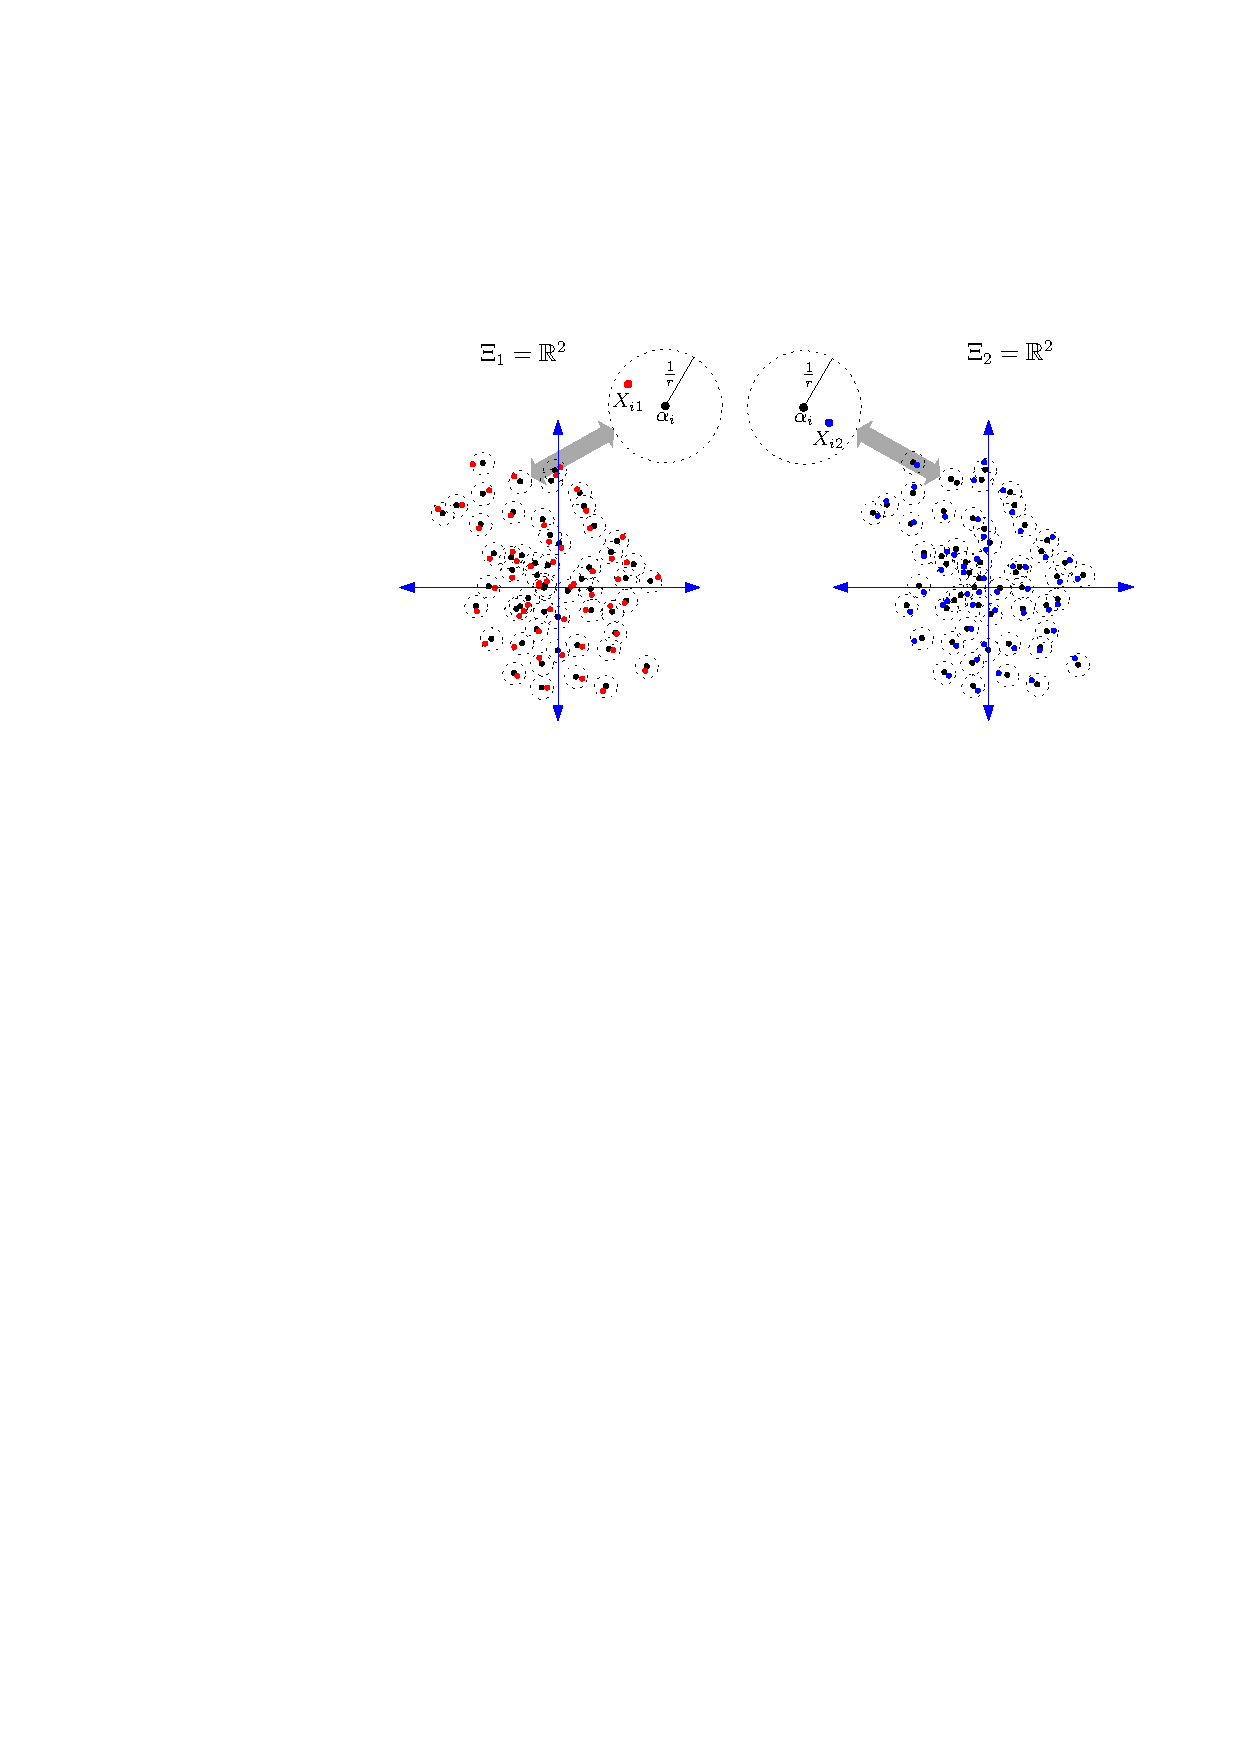
\includegraphics[scale=0.55]{MVN_alpha_r_multiple_sancar.pdf}
    \caption{For the  Gaussian setting (Section \ref{subsec:GaussianSet}), the objects can be represented by $\bm{\alpha_i}$  which are two-dimensional random vectors denoted by black points and distributed as $\mathcal{N}(\bm{0},I_p)$. The dashed lines show the probability contours for each  $\bm{\alpha_i}$. Since  the measurements in the two conditions and the original object   are in the same space (\mathbb{R}^2), $\bm{\alpha_i}$ can be shown along with the measurements the $\bm{x}_{ik}$ which are denoted by red (k=1) and blue (k=2) points respectively.}
\label{fig:Fig1}
	\end{center}
  \end{figure}

% - given the embedded configuration $X$ of the 
%training observations and the augmented dissimilarity matrix that includes dissimilarities between test observations and %the training observations, and dissimilarities in between the training observations, oos-embedding consists of embedding
%the test points into  the existing configuration so as to be as consistent as possible with these dissimilarities (the distances %between points are as close as possible to the dissimilarities as measured by the criterion function). 
\subsection{Simulation\label{subsec:sim}}

We generate the training data of matched sets of measurements (instantiation of $\mathcal{T}$) according to  the Gaussian setting. Dissimilarity representations are computed from pairwise Euclidean distances of these measurements. We also generate a set of matched pairs and unmatched pairs of measurements for testing with the same distribution. Following the out-of-sample embedding of the test dissimilarities 
%(computed via by one of the three P$\circ $M, CCA and JOFC approaches), 
we compute test statistics  for matched and unmatched pairs. This allows us to compute the empirical power  at different $\alpha$ (Type I error rate) values and the empirical AUC measure.


\begin{figure}[h]
     \centering
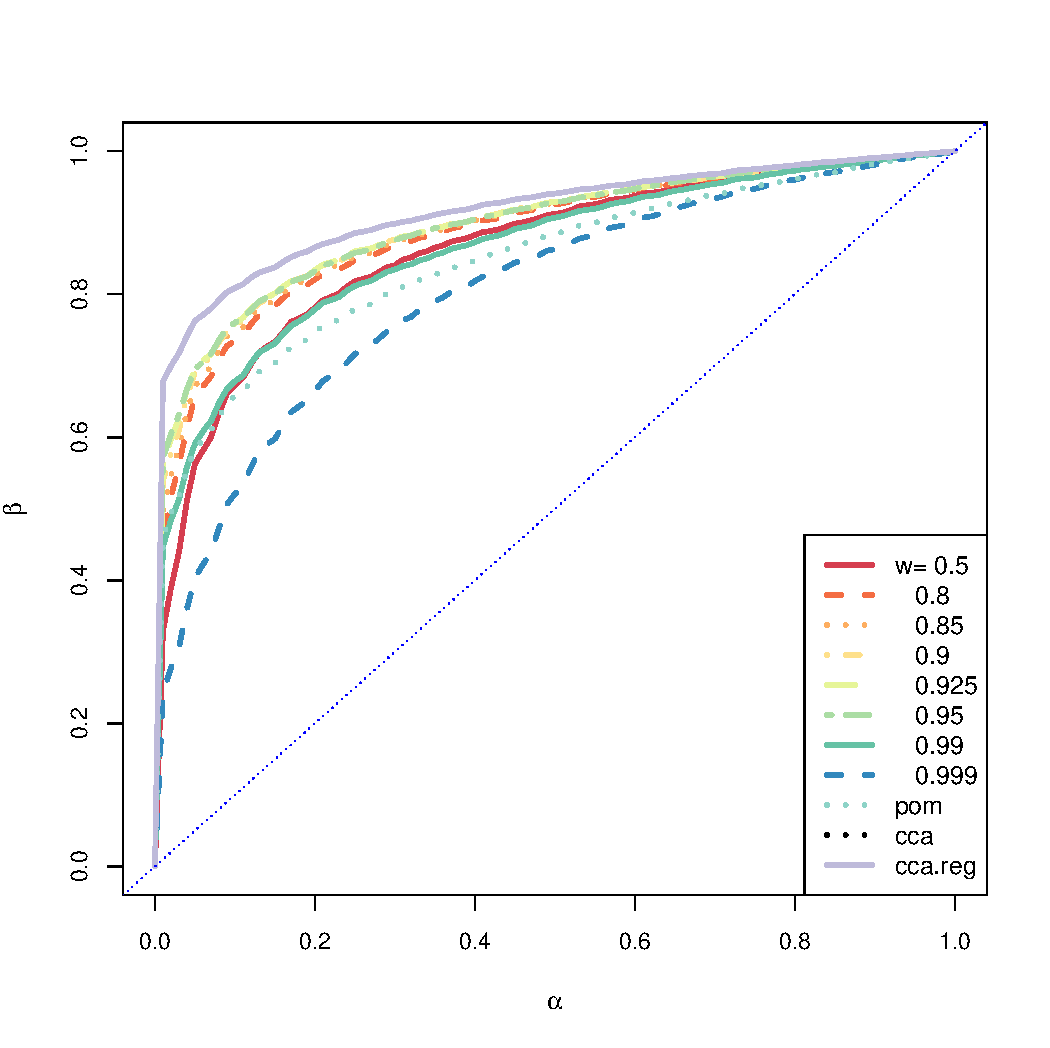
\includegraphics[scale=0.35]{MVN-FC-Tradeoff-OOS-c0.pdf}
\caption{$\beta$ vs $\alpha$  for different $w$ values }
\label{fig:MVN-c0-power-alpha}
\end{figure}

\begin{figure}[h]
  %\captionsetup[subfigure]{subrefformat=parens,labelformat=parens}
      \centering
         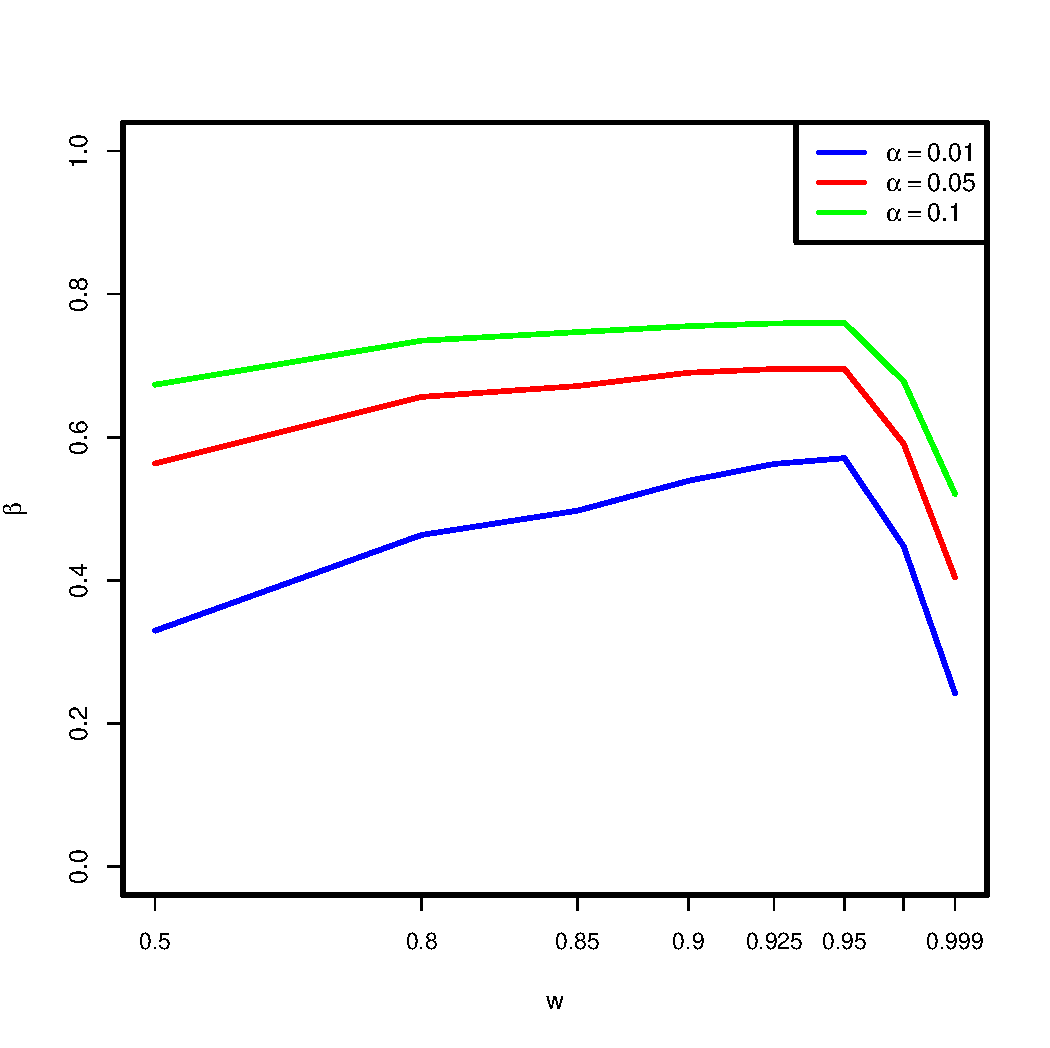
\includegraphics[scale=0.35]{OOSMVN-power-w-c0.pdf}
\caption{$\beta$ vs $w$ plot for different $\alpha$ values }
\label{fig:MVN-c0-power-w}
      

  \end{figure}

\begin{comment}

\begin{figure}
 \centering
  %\captionsetup[subfigure]{subrefformat=parens,labelformat=parens}
       
        \begin{subfigure}[]{0.45\textwidth}        
           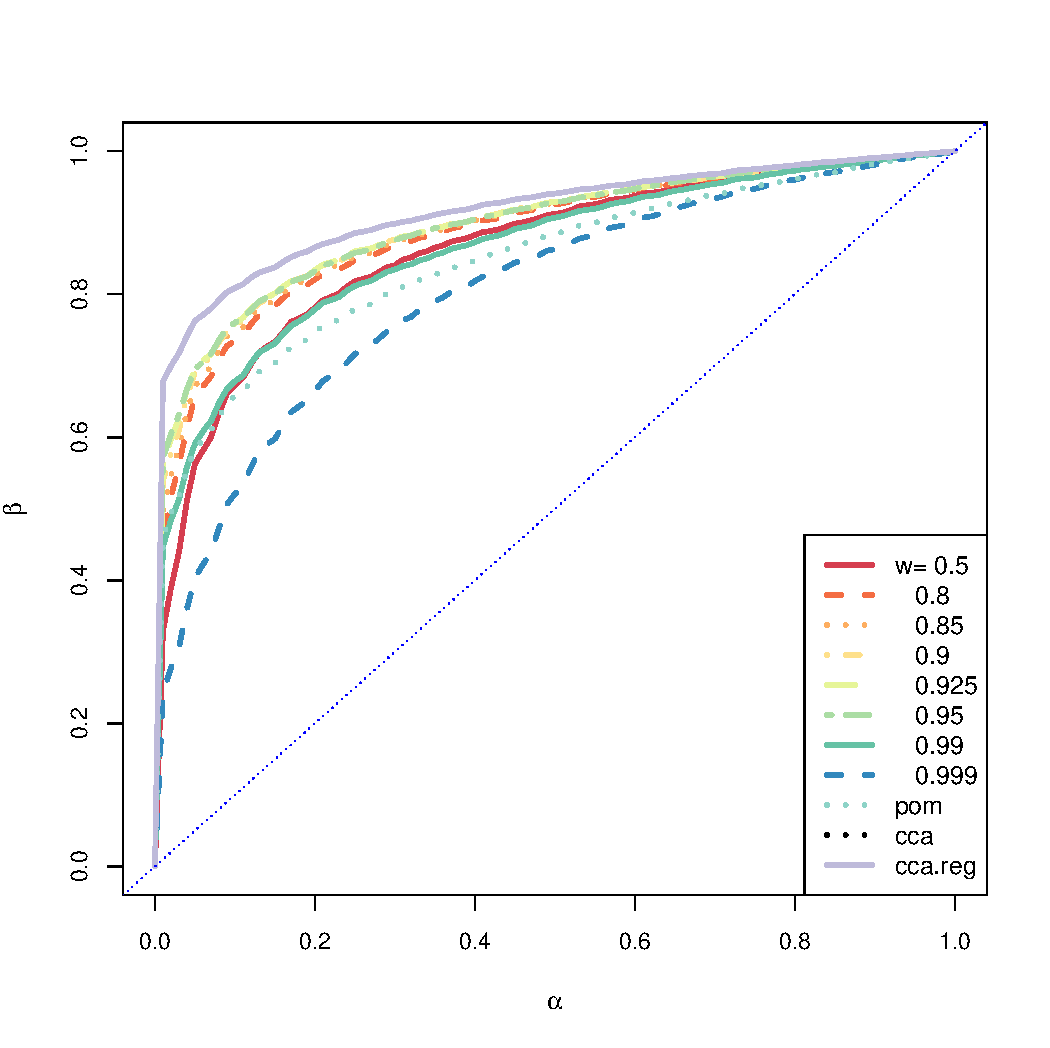
\includegraphics[scale=0.35]{MVN-FC-Tradeoff-OOS-c0.pdf}
\caption{$\beta$ vs $\alpha$  for different $w$ values }
\label{fig:MVN-c0-power-alpha}
        \end{subfigure}%        
         \begin{subfigure}[]{0.45\textwidth}  
         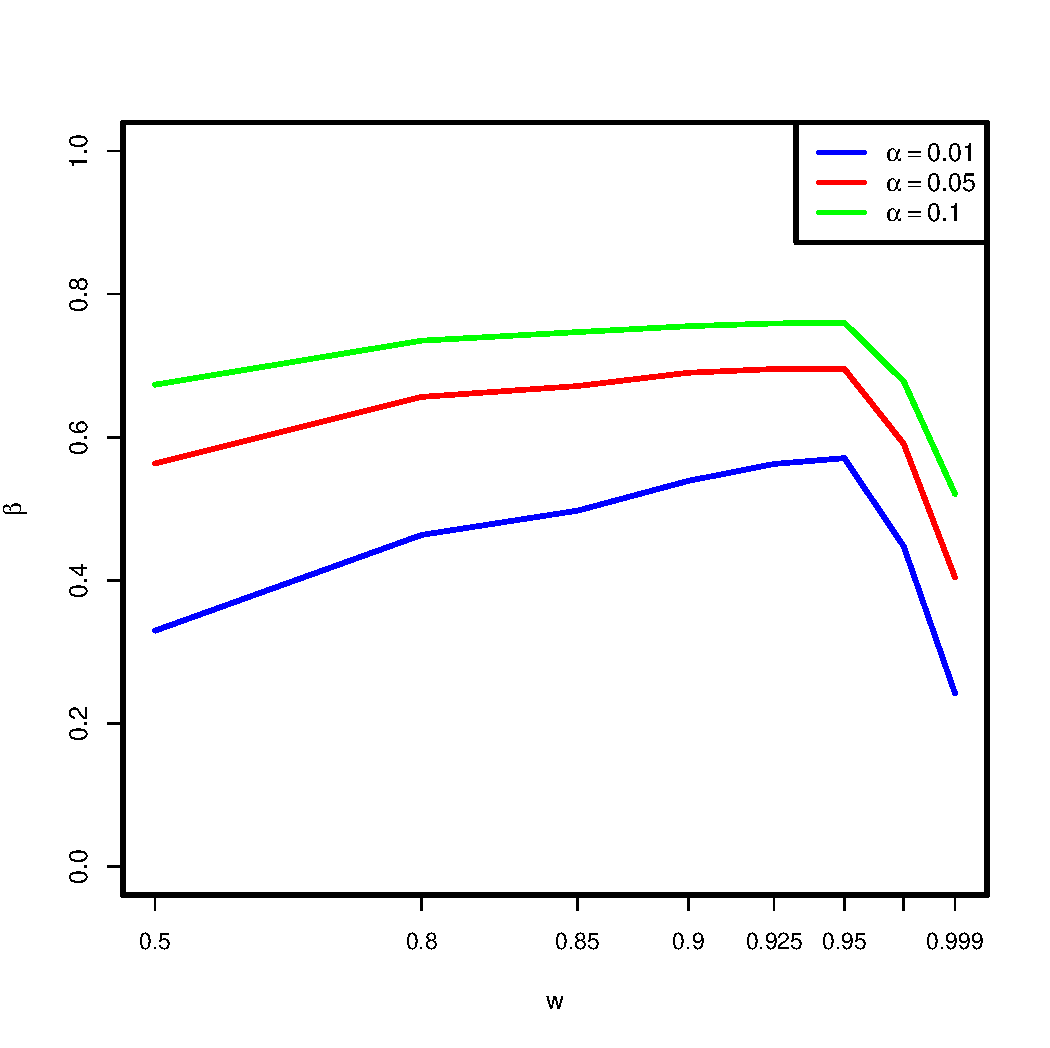
\includegraphics[scale=0.95]{OOSMVN-power-w-c0.pdf}
\caption{$\beta$ vs $w$ plot for different $\alpha$ values }
\label{fig:MVN-c0-power-w}
         \end{subfigure}%
          
  \caption {ROC curves and $\beta$ vs $w$ plots for simulation experiments}
  \end{figure}
	
\end{comment}	
	


%The signal  and noise dimensions ($p$ and $q$) were chosen as 5 and 10, respectively.
 The measurements for the Gaussian setting are vectors in p-dimensional Euclidean space (p=5). For $nmc=150$ Monte Carlo replicates,  $n=150$ matched training pairs and $m=150$ matched and unmatched test pairs (generated according to the Gaussian setting) were generated. Using the resulting test statistic values for matched and unmatched test pairs, the AUC measure was computed for different $w$ values along with the average of the power($\beta$) values at  different $\alpha$s. The plot in Figure \ref{fig:MVN-c0-power-alpha} shows the  $\beta$-$\alpha$ curves for different values of  $w$. In Figure
 \ref{fig:MVN-c0-power-w},  $\beta(w)$ is plotted against $w$ for fixed values of $\alpha$.  
The average AUC measure for these $nmc=150$ MC replicates are  in  Table \ref{tab:AUCW}.

\begin{table}[h]
\centering
\begin{tabular}{rrrrrrrrrrr}
  \hline
$w$ & 0.1 & 0.4 & 0.5 & 0.8 & 0.85 & 0.9 & 0.925 & 0.95 & 0.99 & 0.999 \\ 
  \hline
AUC & 0.811 & 0.822 & 0.834 & 0.886 & 0.896 & 0.902 & 0.902 & 0.898 & 0.849 & 0.782 \\ 
   \hline
\end{tabular}
\caption{average AUC($w$) for $nmc=150$ MC replicates}
	\label{tab:AUCW}
\end{table}


  The $w$ value  which results in the highest $AUC$ measure  is different for each MC replicate.  The number of  MC replicates  for  which a particular $w$ value led to the highest $AUC$ is shown in  the bar chart in 	\ref{fig:ArgMaxWAUCW}. Only the non-zero counts are  shown in \ref{fig:ArgMaxWAUCW}. The estimate $\hat{w}^* $ can be chosen as  as 0.925, as it is the mode of w^* estimates from each MC replicate. We should note that the AUC function is very flat in the interval (0.85,0.99), and it is possible that the difference between the largest value of  $AUC$ measure and the next highest is very small.
\begin{figure}[h]
	\centering
	
		
\includegraphics[scale=0.15]{auc_argmax_hist.pdf}
	
	\caption{Histogram of $\arg\max_w AUC(w)$ for $nmc=150$ replicates}
	\label{fig:ArgMaxWAUCW}
\end{figure}


 %It is  interesting that the optimal value of $w$ seems to be in the range of $(0.85,1)$ for this setting, which suggests a significant emphasis on commensurability might be  critical for the match detection  task. 
%Simulations with other values for  the embedding dimension $d$  resulted in $w^*$ estimates closer to $0.5$. 





\begin{comment}
\begin{figure}
\includegraphics[scale=0.35]{OOS-MVN-power-w-c0.pdf}
\caption{$\beta$ vs $w$ plot for fixed $\alpha$ values for the Gaussian setting (noiseless case)}
\label{fig:MVN-c0-beta-w}
\end{figure}


\begin{figure}
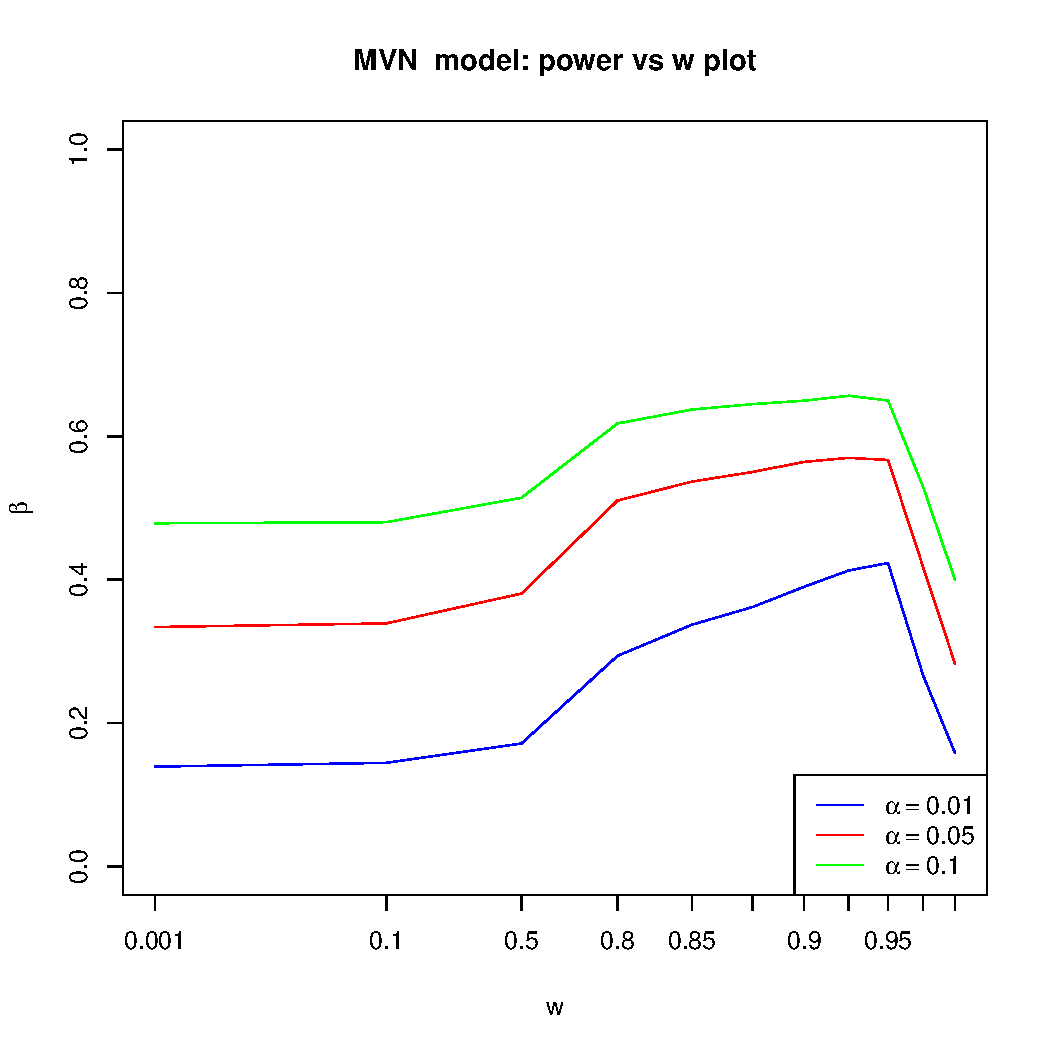
\includegraphics[scale=0.65]{OOSMVN-power-w-c001.pdf}
\caption{Power ($\beta$) vs $w$ plot for fixed Type I error ($\alpha$) values for the Gaussian setting (noisy case)}
\label{fig:MVN-c001-beta-w}
\end{figure}



Note that in Figure \ref{fig:MVN-c001-power-w} for $\alpha=0.05$, $\beta_{\alpha=0.05}(w=0.99)\geq\beta_{\alpha=0.05}(w=0.5)$. However, for $\alpha=0.3$, $\beta_{\alpha=0.3}(w=0.99)\leq\beta_{\alpha=0.3}(w=0.5)$. This justifies our comment that  $w^{*}$  must be defined with respect to $\alpha$.


\begin{figure}
\includegraphics[scale=0.35]{OOS-Dirichlet-power-w-c0.pdf}
\caption{$\beta$ vs $w$ plot for fixed $\alpha$ values for the Dirichlet setting(noiseless case)}
\label{fig:fig7}
\end{figure}

\begin{figure}
\includegraphics[scale=0.35]{OOS-Dirichlet-power-w-c0-01.pdf}
\caption{$\beta$ vs $w$ plot for fixed $\alpha$ values for the Dirichlet setting(noisy case)}
\label{fig:fig8}
\end{figure}
\end{comment}



Note that   the estimate of the optimal $w^{*}$  has  an AUC measure higher than  that of $w$=0.5 (uniform weighting). This finding was confirmed using data generated 
%in different settings, such as  the Dirichlet setting (introduced in \cite{JOFC}) and
according to  the Gaussian setting with different sets of parameters.

\begin{comment}



\section{Model Selection}
For the simulations presented up to now, the embedding dimension $d$ was set to 2. This was a convenient choice which allowed us to investigate various aspects of JOFC and competing approaches.
However,  more care is required in selection of this parameter, since it plays such a big role in performance in general learning settings. The signal dimension was set to $p=10$ and different $d=2,5,7,10,15$ values were used to test the JOFC approach.
The following plots of ROC curves in    \ref{fig:ROC-d} and  \ref{fig:ROC-d-15} shows the effect of $d$ parameter on the performance of different methods for the Gaussian setting for the noisy case. 
\begin{figure}
 \centering
 % \captionsetup[subfigure]{labelformat=empty}
        \begin{subfigure}[b]{0.5\textwidth}        
               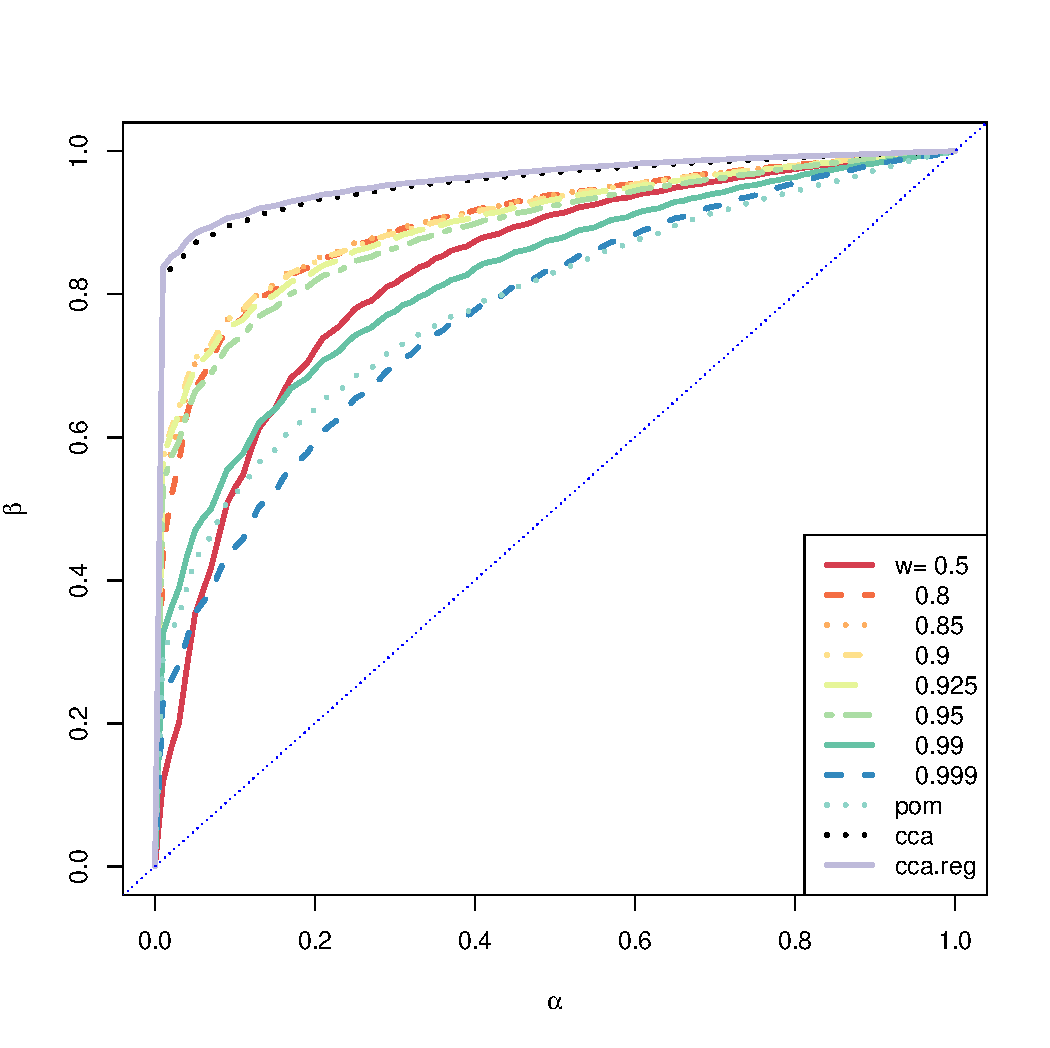
\includegraphics[width=\textwidth]{ROC-d-2.pdf}
                \caption{d=2}
                \label{fig:ROC-d-2}
        \end{subfigure}%
         %add desired spacing between images, e. g. ~, \quad, \qquad etc. 
          %(or a blank line to force the subfigure onto a new line)
        \begin{subfigure}[b]{0.5\textwidth}           
                  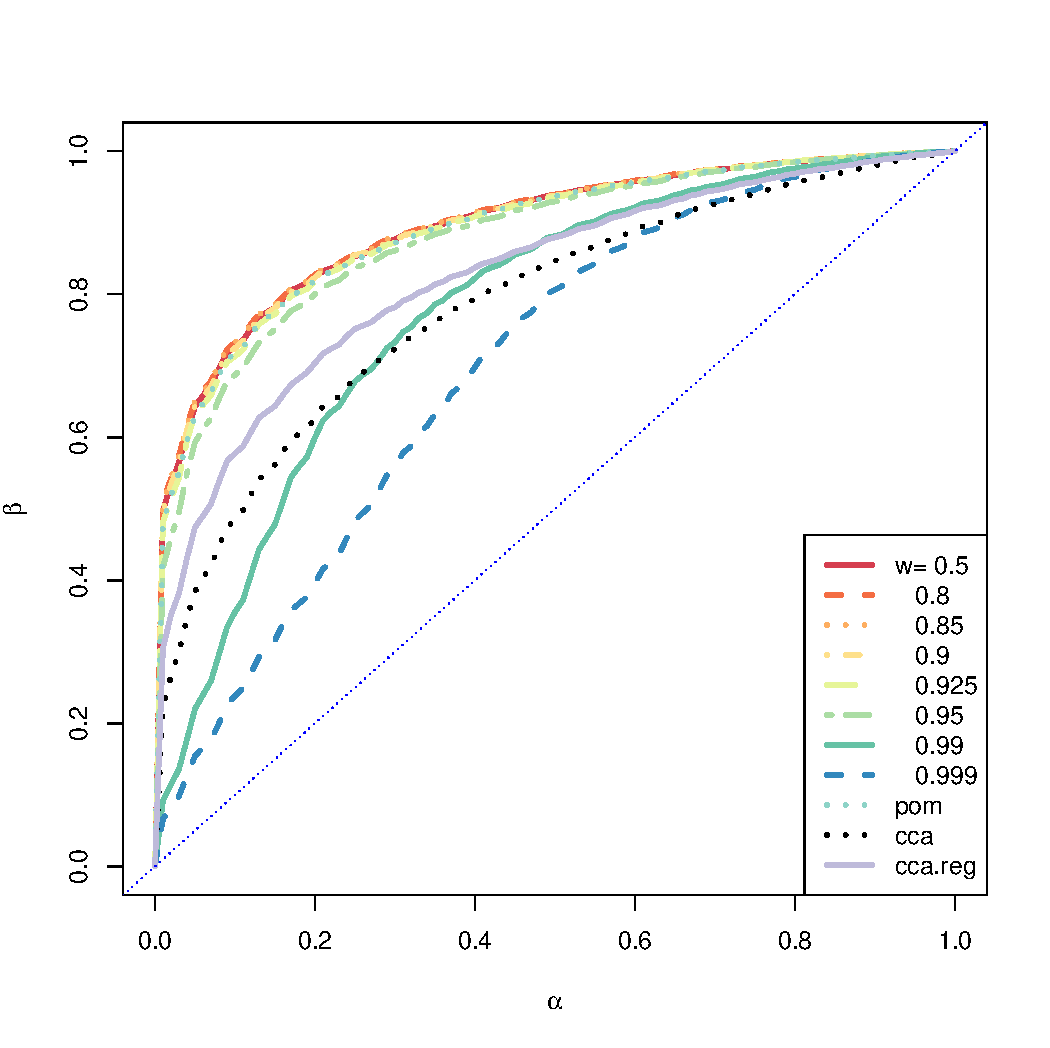
\includegraphics[width=\textwidth]{ROC-d-5.pdf}
                \caption{d=5}
                \label{fig:ROC-d-5}
        \end{subfigure}      
        %add desired spacing between images, e. g. ~, \quad, \qquad etc.    %(or a blank line to force the subfigure onto a new line)
        \begin{subfigure}[b]{0.47\textwidth}             
               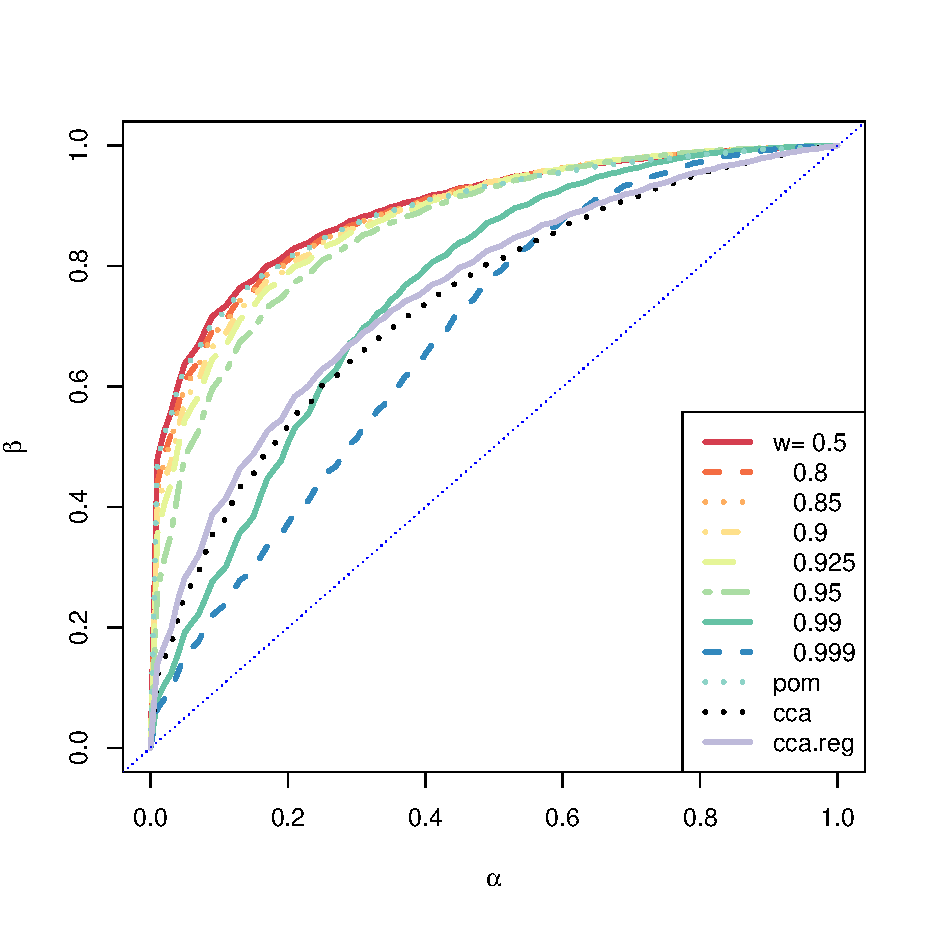
\includegraphics[width=\textwidth]{ROC-d-7.pdf}
                \caption{d=7}
                \label{fig:ROC-d-7}
        \end{subfigure}          
               \begin{subfigure}[b]{0.47\textwidth}
                \centering
               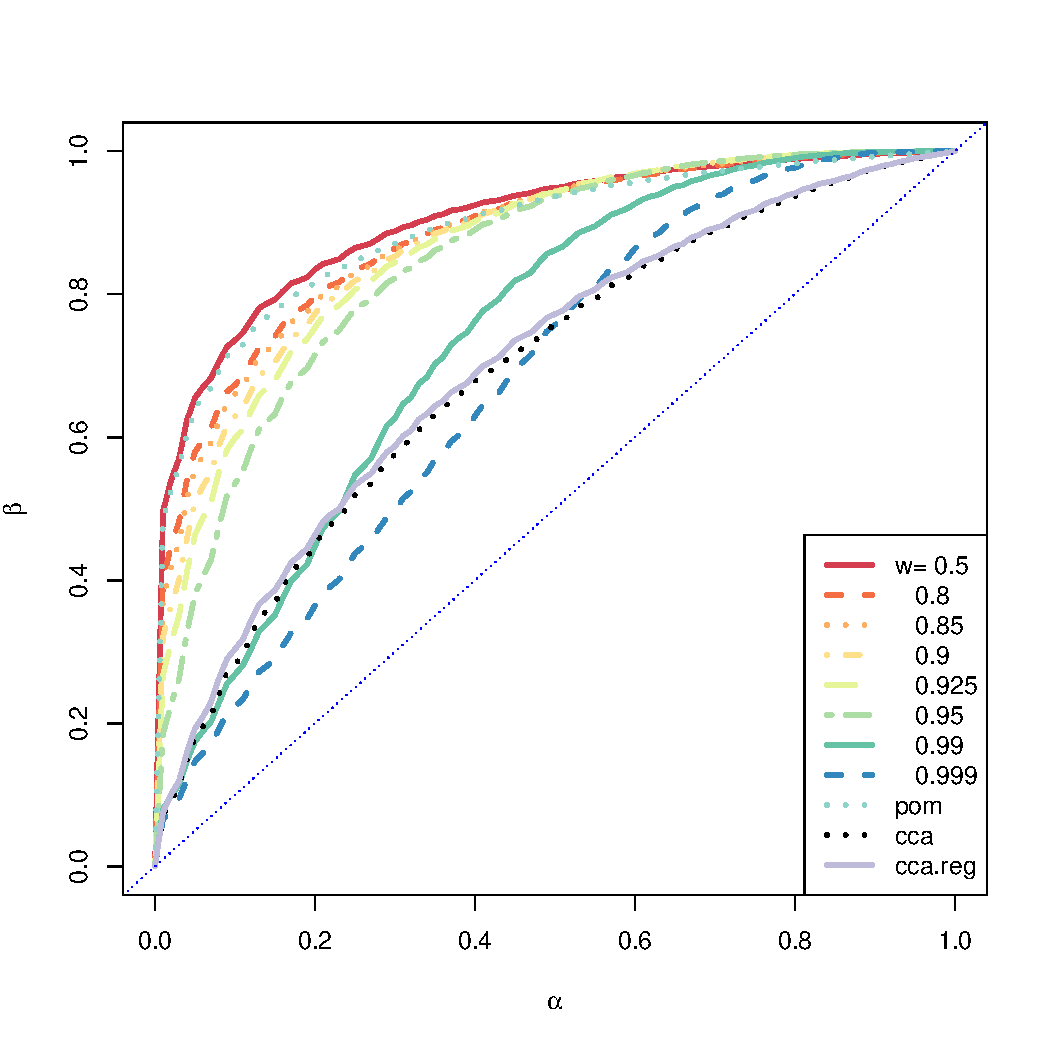
\includegraphics[width=\textwidth]{ROC-d-10.pdf}
                \caption{d=10}
                \label{fig:ROC-d-10}
        \end{subfigure}
        
          \begin{subfigure}[b]{0.47\textwidth}
             \centering
               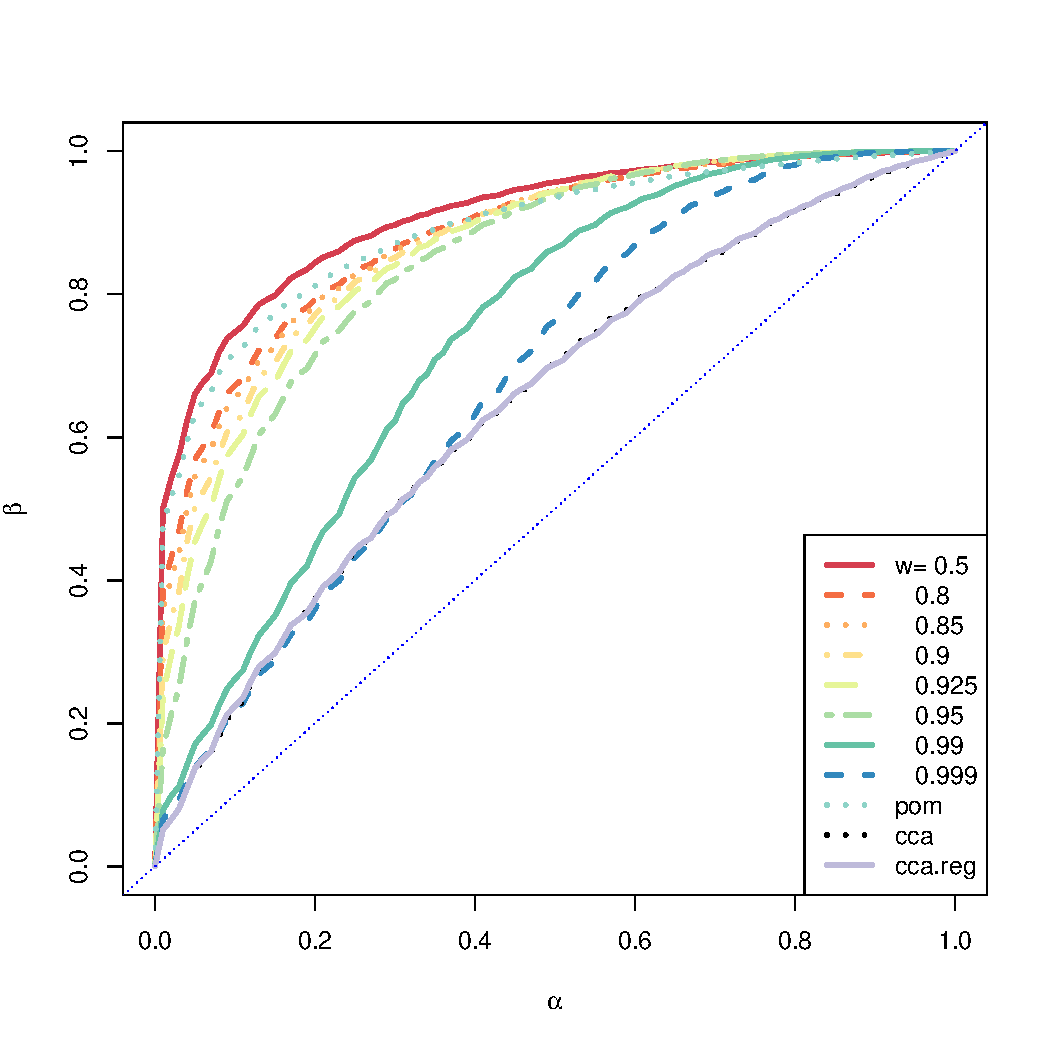
\includegraphics[scale=0.3]{ROC-d-15.pdf}
                \caption{d=15}
                \label{fig:ROC-d-15}
                        \end{subfigure}
         
        \caption{Effect of $d$ parameter on ROC plots}\label{fig:ROC-d}
        \label{fig:ROC-d}

\end{figure}


\end{comment}

\section{Conclusion}
 The tradeoff between Fidelity and Commensurability and the relation to the weighted raw stress criterion for MDS were both investigated with simulations .
   For  hypothesis testing as the exploitation task, the three approaches were compared in terms of testing power.
    The results indicate that when doing a joint optimization, one should consider an optimal compromise point between Fidelity and Commensurability,
       which corresponds to an optimal weight $w^*$ of the weighted raw stress criterion in contrast to the uniform weighting 
        for omnibus matrix embedding. 
        


\bibliographystyle{plain}
\bibliography{priebe-thesis-JOFC}



\end{document}
